
\documentclass[10pt,letterpaper]{article}

\usepackage{cogsci}
\usepackage{amsmath}
\usepackage{bm}
\usepackage{graphicx}
\usepackage{subcaption}

\usepackage{epigraph}
\setlength\epigraphrule{0pt}

%\cogscifinalcopy % Uncomment this line for the final submission 

\usepackage[dvipsnames]{xcolor}
\usepackage{pslatex}
\usepackage{apacite}
\usepackage{float} % Roger Levy added this and changed figure/table
                   % placement to [H] for conformity to Word template,
                   % though floating tables and figures to top is
                   % still generally recommended!

%\usepackage[none]{hyphenat} % Sometimes it can be useful to turn off
%hyphenation for purposes such as spell checking of the resulting
%PDF.  Uncomment this block to turn off hyphenation.


%\setlength\titlebox{7.5cm}
% You can expand the titlebox if you need extra space
% to show all the authors. Please do not make the titlebox
% smaller than 4.5cm (the original size).
%%If you do, we reserve the right to require you to change it back in
%%the camera-ready version, which could interfere with the timely
%%appearance of your paper in the Proceedings.


% Not sure if we want to change this title
\title{The Art of (Recursive Bayesian) Persuasion}
 
\author{{\large \bf Samuel A. Barnett (samuelab@princeton.edu)} \\
  Department of Computer Science, Princeton University \\
  Princeton, NJ 08540 USA  
\AND {\large \bf Robert X. D. Hawkins (rdhawkins@princeton.edu)} \\
  Department of Psychology, Princeton University \\
  Princeton, NJ 08540 USA
\AND {\large \bf Mark K. Ho (mho@princeton.edu)} \\
  Department of Psychology, Princeton University \\
  Princeton, NJ 08540 USA
\AND {\large \bf Thomas L. Griffiths (tomg@princeton.edu)} \\
  Department of Psychology, Princeton University \\
  Princeton, NJ 08540 USA}


\begin{document}

\maketitle


\begin{abstract}
An honest speaker that is attempting to convince you of some fact must balance
the need to be show the strongest evidence for that fact with the need to appear as an impartial informer. An effective listener
will be able to make inferences from a biased speaker if also modeling the fact that
the speaker has a bias of some nature. Here, we employ a recursive Bayesian model
of two particular phenomena that arise in this context: the weak and strong evidence effects.
We show that the model is capable of capturing these effects in an intuitive way, and that the
higher-order levels of reasoning are \textit{essential} for doing so.

\textbf{Keywords:} 
communication; computational modeling; persuasion; rational analysis; theory of mind
\end{abstract}

\section{Introduction}
\begin{epigraphs}
\qitem{There are, then, these three means of effecting persuasion [...] (1) to reason logically, 
(2) to understand human character and goodness in their various forms, and (3) to understand 
the emotions}{\textit{Aristotle}}
\qitem{Well he would [say that], wouldn't he?}{\textit{Mandy Rice-Davies}}
\end{epigraphs}

% Motivate the problem. 
Much of the information we learn comes through communication with actors 
in the world with their own desires, model of the world, and epistemological access to it. An honest speaker 
that is attempting to convince you of some fact must balance the need to show you
the evidence that best supports her case
with the need to appear as an impartial informer. An effective listener will be able to 
make inferences from a biased speaker, regarding both the bias of the speaker and the
content of his utterances.

\textcolor{red}{Tom: Spend a moment on the big picture modeling challenge before getting into specific phenomena.}

% Describe the strong and weak evidence effect. Talk about relevant papers.
This paper models two particular phenomena that occur in the context of communication
with biased speakers: the \textit{weak} and \textit{strong evidence effects}. 

The \textit{weak evidence effect} typically occurs in the context in which a listener first
hears one side of a dispute, followed by the other side \cite{mckenzie_when_2002}.  For example, in a courtroom, jurors first
hear the plaintiff's case, followed by the defendant's case. If the plaintiff makes a strong case, then
a subsequently weak case made by the defendant may make the jurors \textit{more} confident in the 
plaintiff's case. This is intuitive from a pragmatic perspective: the jurors expect both the plaintiff and 
defendant to present the strongest arguments for their case, and so the weakness of the defendant's
case suggests an absence of stronger evidence. However, on a na\"ive model in which we do not
consider how the evidence is selected, it would be inconsistent to reduce one's confidence in the
defendant's case on hearing her argument, if the argument on its own raises the probability of her
side being true \cite{fernbach_when_2011}.

The \textit{strong evidence effect}, in contrast, shows how stronger evidence may not always lead
to stronger inferences \cite{perfors_stronger_2018}. In particular, knowing that a speaker's utterances will be used to make inferences
about bias can lead to a speaker modulating the evidence she presents to a listener, rather than presenting
the strongest possible argument for her case. This has been found to occur even when the distribution
of the underlying evidence leans overwhelmingly towards the speaker's side of the argument.

% Say how you'll model these. 
This paper shows how both the strong and weak evidence effects can be predicted and explained under
one unified Bayesian computational model in the toy context of \textit{the stick task}. 
Simulation 1 is based on experiments in \citeA{mckenzie_when_2002}, and Simulations 2 and 3 are based on
Studies 1 and 2 in \citeA{perfors_stronger_2018}, respectively.
This is the first computational model to demonstrate the 
strong evidence effect, and the first model of the weak evidence effect employing an explicit theory of mind
in its explanation.\footnote{Previous work models the weak evidence effect by evaluating case strength with
respect to a malleable reference point. Furthermore, faint praise, a phenomenon related to the weak evidence effect,
has been given a Bayesian formalization by \citeA{harris_james_2013}.}

The core of this model is recursive Bayesian inference about underlying states given utterances by Bayesian
decision-makers, in the style of Rational Speech Act (RSA) models \cite{goodman_pragmatic_2016}. In particular, we begin at the lowest level
with a na\"ive judge who assumes the evidence he receives is impartial, and add alternate layers of speakers
and judges in order to capture higher-order reasoning about the best means of persuasion. The agenda
of each speaker can then be captured by a simple, scalar bias parameter.

% Briefly summarise results.
The results from this paper show that the recursive Bayesian model of persuasion is able to capture both the
weak and strong evidence effects. Moreover, the higher-order models of speakers and listeners are shown to
be \textit{essential} for capturing the effect, thus justifying the framework under which this model is designed. 
Finally, we show that varying parameters such as the speaker bias, or the way in which this bias is perceived by
the judge, changes the nature of the weak and strong evidence effects in intuitive ways.

\section{Background}
% Describe weak, strong, and pedagogical sampling as related work.
This work is also related to work about learning from examples showing that different assumptions
about how the data are sampled can have a large impact on learning. In particular, previous models have 
looked at \textit{weak}, \textit{strong}, and \textit{pedagogical} sampling 
\cite{hsu2009differential, shafto_rational_2014, tenenbaum1999bayesian, tenenbaum2001generalization}, each corresponding to different ways
in which the data are generated, and subsequently corresponding to different likelihood functions assumed by
the learner. This work can be considered to introduce a fourth sampling assumption, \textit{rhetorical sampling},
in which the data are generated by a speaker who is trying to convince the learner of her point of view, which
also appears in the learner's likelihood function.\footnote{A related model in which the agents are allowed to \textit{deceive}
a listener is considered in \citeA{oey_designing_2019}.	}

\section{Modeling Evidence Effects}
\subsection{World Model: The Stick Task}
We model the weak and strong evidence effects on a simple toy task called \textit{the stick task}.
In this task, a judge must reason about the mean of a sample originally drawn from a known distribution,
where observations from the sample are presented by biased agents.

% Introduce the notation and describe the objective of the stick task.
In particular, the stick task consists of a judge, and a set of speakers indexed by $I$. 
A sample of $N$ sticks whose lengths are given by
\begin{equation}
\mathcal{S}_N = \{ s_1, s_2, ..., s_N \}
\end{equation}
are drawn i.i.d.\ from the Uniform$[0,1]$ distribution and is fixed throughout
the task.\footnote{In practice, we use a discrete approximation to this distribution 
by modeling the sticks as being drawn uniformly from the set~${\{ 0.025, 0.075, ..., 0.975\}}$.} 

Each speaker observes the full sample before the task, and at each time step $t$ a speaker
$i$ (one per time step, taking it in turn) chooses one stick from the sample to reveal
to the judge. The speakers are not permitted to reveal a stick that has previously been shown to 
the judge. Notationally, the speaker chooses action 
\begin{equation}
a_t^{(i)} \in \{s_1, s_2, ..., s_N\} \setminus \mathcal{A}_{t-1},
\end{equation}
where $s_i$ is the realization of random variable $S_i$ and $\mathcal{A}_{t-1}$ denotes the first~${t-1}$ 
actions chosen. For simplicity, we let~${\mathcal{A}_0 = \emptyset}$.

At each time step $t$, the judge reasons about the sample mean of the sticks,~${\bar{S} = \frac{1}{N} \sum_{n=1}^N s_n}$.\footnote{It is assumed that the judge knows $N$, but only observes the stick values through the speakers' actions.}
In particular, the judge evaluates his posterior over whether the sample is `long' or `short', i.e., whether or not
$\bar{S	}_N \ge 0.5$. Hence, the relevant posterior for the judge at time step $t$ is
\begin{equation}
p( \bar{S}_N \ge 0.5 \ | \ \mathcal{A}_t ).
\end{equation}

Each speaker will have an incentive to select evidence that persuades the judge that the sample is
either long or short, or the speaker will be indifferent towards the outcome. Observe that, for the above posterior, 
the length of each stick observed is directly proportional to the strength of the belief that the sample is long.
This direct correlation allows us to clearly model the weak and strong evidence effect by treating the
length of each stick as a proxy for the strength of the evidence supporting the statement.

The task runs for a total of~${T\le N}$ time steps.

\subsection{Agent Models}
In the manner of Rational Speech Act (RSA) models \cite{goodman_pragmatic_2016}, we model the speakers as performing
recursive Bayesian inference about one another's beliefs. To capture both evidence effects,
we require four layers, which we divide into the `na\"ive' layers and the `pragmatic' layers.
The model is implemented in WebPPL \cite{dippl}, a probabilistic programming language that allows for
fast hierarchical inference in low-dimensional domains such as this one.

\subsubsection{Na\"ive Judge and Speaker}
The first layer, $J_0$, describes the na\"ive judge - this judge is na\"ive in the sense that he
does not model the speakers as having any incentives, and instead assumes that the actions are selected
uniformly from the available sample. Relabeling without loss of generality, the posterior of $J_0$ at time $t$ is given by
\begin{equation}
p_{J_0}( \bar{S}_N \ge 0.5 \ | \ s_1, s_2, ..., s_t).
\end{equation}

The second layer, $S_1$, describes the na\"ive speaker, whose choice about which stick to show
at time $t$ is represented as a posterior over the available sticks defined in reference to $p_{J0}$.
Importantly, each speaker has a bias $\beta$, where in our simulations we model the biases as being
in the range~${\beta \in \{-10, -5, -2, 0, 2, 5, 10\}}$. This bias represents the incentive regarding the judge's
inference: a positive (resp. negative) bias entails that the speaker is incentivized to show sticks to the judge
that steer the judge towards the belief that the sample is long (resp. short).

To produce this behavior, the speaker samples a stick based on the soft-maximization of biased informativity
of that stick, taking into account the previous sticks shown. If~${\beta\ge 0}$, then this is written as:
\begin{equation}\label{S1}
p_{S_1} (a_t \ | \ \mathcal{A}_{t-1},\ \mathcal{S}_N, \beta) \propto \exp \bigl(\lvert\beta\rvert \cdot p_{J_0} (\bar{S}_N \ge 0.5 \ | \ \mathcal{A}_{t-1} \cup \{a_t\} \bigr).
\end{equation}

For $\beta<0$, we simply replace the event~${\bar{S}_N \ge 0.5}$ in the above expression with~${\bar{S}_N < 0.5}$.
Observe that, if $\beta = 0$, this entails that the speaker will sample the sticks uniformly based on the available
evidence, which is equivalent to the speaker being indifferent to the outcome.\footnote{The $\beta$ parameter also 
plays the same role as the optimality parameter $\alpha$ in models such as that of \citeA{goodman_pragmatic_2016}.}

\subsubsection{Pragmatic Judge and Speaker}
The pragmatic judge, $J_1$, performs a similar inference as $J_0$, though with one crucial difference: the judge
models each stick as having been sampled by a na\"ive speaker. To see how this is possible, observe that we can express
the action of speaker $i$ at time $t$ by the random variable 
\begin{equation}
	A_t^{(i)} \sim p_{S_1} (\cdot \ | \ \mathcal{A}_{t-1},\ \mathcal{S}_N),
\end{equation}
which is a categorical distribution computed by Equation~\ref{S1}. For ease of notation, we write the set
of observations of $S_1$ speakers
\begin{equation}
	\mathcal{A}'_T = \{ A_1^{(i_1)}=a_1^{(i_1)}, A_2^{(i_2)}=a_2^{(i_2)}, ..., A_T^{(i_T)}=a_T^{(i_T)}\}, 
\end{equation}
and let $\mathcal{A}'_0 = \emptyset$.

In order for the pragmatic judge to reason about the na\"ive speaker, the posterior of $J_1$ must reflect the agent
biases (denoted $\bm{\beta}$) as well as the distribution over remaining sticks. This can be computed by Bayes' rule:
\begin{align*}
	p_{J_1} (\mathcal{S}_N, \bm{\beta} \ | \ \mathcal{A}'_T) &\propto p(\mathcal{A}'_T \ | \ \mathcal{S}_N, \bm{\beta}) p(\mathcal{S}_N) p(\bm{\beta}) \\
	&= p(\bm{\beta}) p(\mathcal{S}_N) \prod_{t=1}^T p_{S_1}(A_t^{(i_t)}=a_t^{(i_t)} \ |  \mathcal{A}'_{t-1}, \bm{\beta})
\end{align*}

Using the sum rule, we arrive at the relevant posterior, which in the case of discretized stick lengths is given by
\begin{equation}
	p_{J_1} ( \bar{S}_N \ge 0.5 \ | \ \mathcal{A}'_T ) = \sum_{\bm{\beta}} \sum_{\substack{\mathcal{S}_N \\ \bar{S}_N \ge 0.5}} p_{J_1} (\mathcal{S}_N \ | \ \mathcal{A}'_T).
\end{equation}

We consider two distinct versions of the pragmatic judge: one in which he knows the biases of each speaker in advance, and
one in which these biases are drawn, i.i.d., from a categorical prior over the aforementioned range of bias values. This is 
necessary as the weak and strong evidence effects demand the former and latter versions, respectively. Given the above notation,
we can view the former case as modeling $p(\bm{\beta})$ as a delta distribution on the known bias values of each speaker.

We further divided the latter case into two by considering two possible priors: a flat prior over the bias range, and a `V-shaped' prior which down-weights 
the likelihood of neutrality.\footnote{Concretely, the V-shaped prior is given by the normalized probability vector $\frac{1}{29} (8, 4, 2, 1, 2, 4, 8)$.} 
We considered these two priors as, although the V-shaped prior better describes the context of the stick task, we wished to show 
that strong evidence effects varied with respect to our choice of prior.

The final layer, the pragmatic speaker $S_2$, is nearly identical to the na\"ive speaker $S_1$, except for the fact that
the pragmatic speaker performs soft-maximization based on $J_1$'s judgment, as opposed to $J_0$'s judgment. For~${\beta\ge0}$,
this is given as
\begin{equation}
	p_{S_2} (a_t \ | \ \mathcal{A}_{t-1},\ \mathcal{S}_N, \beta) \propto \exp \bigl(\lvert\beta\rvert  \cdot p_{J_1} (\bar{S}_N \ge 0.5 \ | \ \mathcal{A}_{t-1} \cup \{a_t\} \bigr),
\end{equation}
with the expression for~${\beta<0}$ changing as for $S_1$.

This layer is only applicable to the simulations capturing the strong evidence effects.

\section{Simulations}
\subsection{Simulation 1: Weak Evidence Effect}
\begin{figure*}[h]
\centering
\begin{subfigure}{0.3\linewidth}
	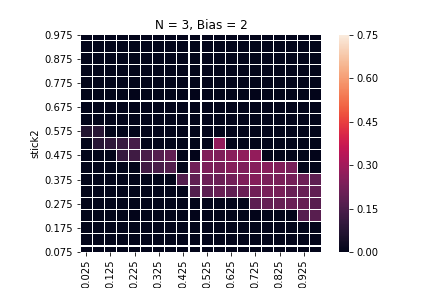
\includegraphics[width=\linewidth]{figures/nSticks3bias2.png}
\end{subfigure}
~
\begin{subfigure}{0.3\linewidth}
	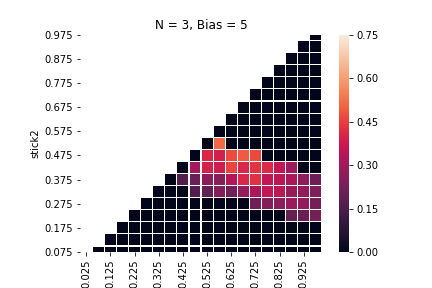
\includegraphics[width=\linewidth]{figures/nSticks3bias5.png}
\end{subfigure}
~
\begin{subfigure}{0.3\linewidth}
	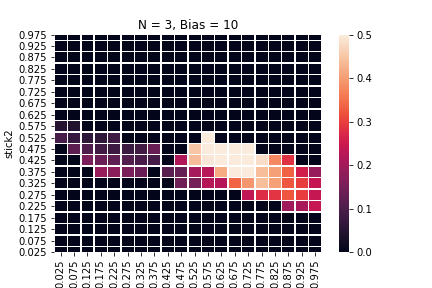
\includegraphics[width=\linewidth]{figures/nSticks3bias10.png}
\end{subfigure}

\begin{subfigure}{0.3\linewidth}
	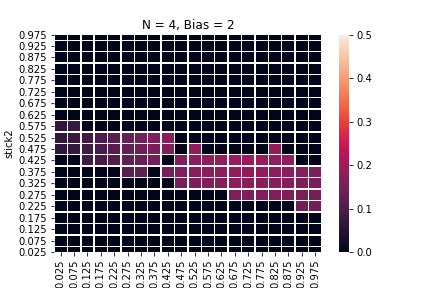
\includegraphics[width=\linewidth]{figures/nSticks4bias2.png}
\end{subfigure}
~
\begin{subfigure}{0.3\linewidth}
	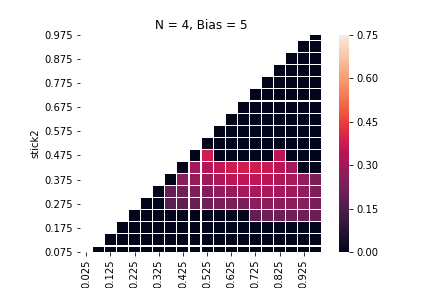
\includegraphics[width=\linewidth]{figures/nSticks4bias5.png}
\end{subfigure}
~
\begin{subfigure}{0.3\linewidth}
	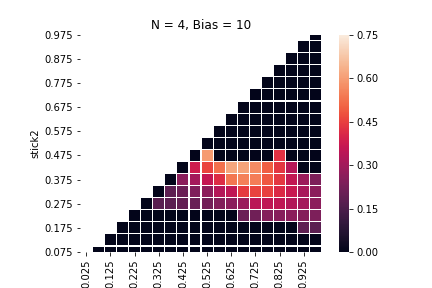
\includegraphics[width=\linewidth]{figures/nSticks4bias10.png}
\end{subfigure}

\begin{subfigure}{0.3\linewidth}
	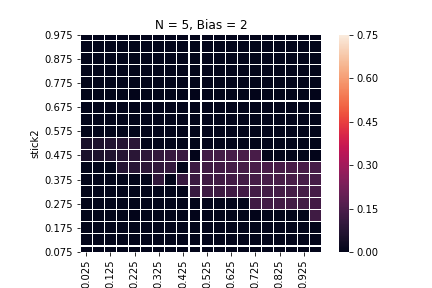
\includegraphics[width=\linewidth]{figures/nSticks5bias2.png}
\end{subfigure}
~
\begin{subfigure}{0.3\linewidth}
	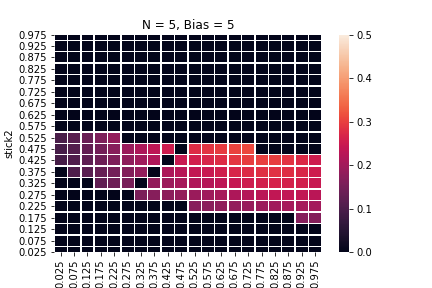
\includegraphics[width=\linewidth]{figures/nSticks5bias5.png}
\end{subfigure}
~
\begin{subfigure}{0.3\linewidth}
	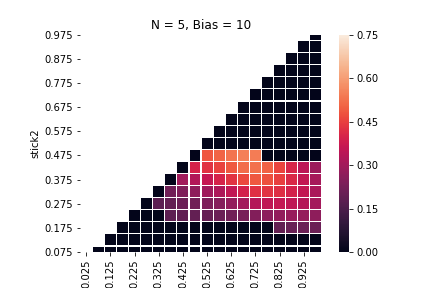
\includegraphics[width=\linewidth]{figures/nSticks5bias10.png}
\end{subfigure}
\caption{Heatmaps depicting the stick pairs for which the weak evidence effect appears, and the strength
of the effect in the cases where it does appear. Values for which there is no weak evidence effect are colored
in black. We vary both the sample size $N$ and the agents' bias strength $\beta$.} 
\label{fig:wee}
\end{figure*}

\subsubsection{Set-Up}
In the first simulation, we captured the pragmatic judge's ability to capture the \textit{weak evidence effect}. We 
present the judge with one stick in turn from two speakers, whose biases are known to the judge and fixed at
\begin{equation}
\beta_1 \in \{2, 5, 10\}, \quad \beta_2 = -\beta_1.
\end{equation}
We then contrast the na\"ive and pragmatic judge's posteriors over whether the
sample is long, having seen both sticks.

In this context, the weak evidence effect occurs when the na\"ive judge \textit{decreases} his belief that the sample is
long between observing the first and the second stick, while the pragmatic judge \textit{increases} his belief. To see
why this is the case, recall that the weak evidence effect is a result of a conditional probability being judged lower than the 
marginal, while the cause is probability-raising. In the stick task, we evaluate whether the cause is probability-raising with
respect to a na\"ive judge, who effectively regards the sticks as being sampled i.i.d., whereas the `conditional' and `marginal' in question
(that is, the conditional probabilities after the first and second stick observation) are evaluated with respect to the pragmatic 
judge with a more nuanced sampling assumption.

We also measure the \textit{strength} of the weak evidence effect for each stick pairing, given by the changes in
belief from observing the first and second stick, summed over the na\"ive and pragmatic judge.\footnote{This is 
set to zero for stick pairings for which the weak evidence effect does not occur.} In particular, this strength is given
by
\begin{equation}
\sum_{J \in \{J_0, J_1\}} \lvert p_J ( \bar{S}_N \ge 0.5 \ | \ \mathcal{A}'_2) - p_J ( \bar{S}_N \ge 0.5 \ | \ \mathcal{A}'_1) \rvert .
\end{equation}

For this simulation, we vary the total sample size $N$ between 3 and 5, and we present to the judge the simplex of possible stick pairs 
where the length of the second stick does not exceed the length of the first.

\subsubsection{Results}
The heatmaps (Fig.~\ref{fig:wee}) show that our model is capable of capturing the weak evidence effect, with the effect being at its 
strongest for~${a_1^{(1)} \approx 0.675}$ and~${a_2^{(2)} \approx 0.47}$. Notably, this effect seems to \textit{weaken} for
stronger values of $a_1^{(1)}$: this is possibly due to the fact that such strong evidence makes it very unlikely that
the sample is short, so that the weaker evidence causes a smaller shift in belief for both judges.

We also observe that increasing the magnitude of the biases for both speakers increases both the range 
of stick pairs for which we observe the weak evidence effect, as well as the strength of the effect. That this occurs is
no surprise: in the limit, observations of sticks from biased speakers effectively inform us of the upper and lower bounds
of the sample, giving us a significant amount of information about the sample mean in the case in which the second stick
provides weak evidence for the sample being short.

Finally, we see that increasing the sample size broadens the range of stick pairs for which we observe the weak evidence
effect.


\subsection{Simulation 2: Strong Evidence Effect for Judges}
\begin{figure*}[h]
\centering
\begin{subfigure}{0.45\textwidth}
	\centering
	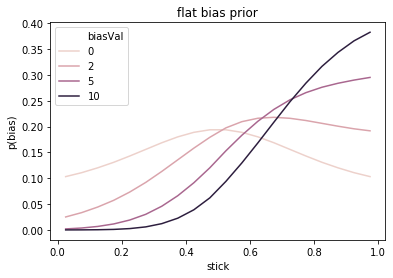
\includegraphics[width=\textwidth]{figures/seeFlat.png}
\end{subfigure}
~
\begin{subfigure}{0.45\textwidth}
	\centering
	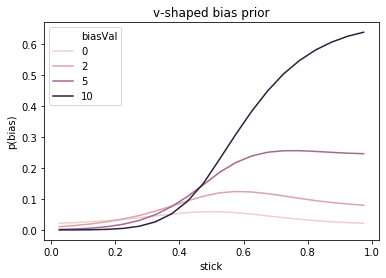
\includegraphics[width=\textwidth]{figures/seeV.png}
\end{subfigure}
\caption{Pragmatic judge $J_1$'s posterior over agent bias, after seeing one stick, where the stick length
and initial prior shape are varied.} 
\label{seeJudge}
\end{figure*}

\subsubsection{Set-Up}
In this simulation, we investigate the strong evidence effect for \textit{judges}, which predicts a relationship between 
the strength of the evidence presented by a speaker, and the judge's perception of the speaker's bias.
We again consider one speaker, and look at the judge's posterior probability of the speaker's bias value after 
observing one stick, where this distribution is computed exactly via enumeration.\footnote{Clearly, the judge does 
not know \textit{a priori} what the speaker's bias value is in this context, in contrast to Simulation 1.} We also vary 
whether the judge begins with a flat prior over bias values, or a V-shaped prior.

\subsubsection{Results}

Fig.~\ref{seeJudge} shows, predictably, that an increased stick length leads to an increased posterior probability in
higher bias values, whereas for lower bias values this increase eventually plateaus or slightly decreases. This is clearer 
in the case of a flat bias prior than a V-shaped prior, where the initial skew in belief towards greater bias values suppresses
the belief that the speaker is positively biased for lower stick values. However, in both cases the overall shape and trend 
of the curves are the same.

\section{Experiment}
To evaluate our model, we implemented a version of the stick task that could be played by a human judge responding to
stimuli from two `contestant' speakers. This allowed us to test whether the weak evidence effect and the strong evidence effect
for listeners was present in the stick task, and whether the model could predict the strength of the effect and the circumstances
under which it occurs.

\subsection{Procedure}
$X$ participants were recruited via MTurk to participant in our experiment using \texttt{nosub}. Participants were briefed
that they were to be the judge of a debate between two contestants, one of which would be rewarded \$10 based on the participant's
final judgment about the sample. In order to be included in the trial, they must successfully complete a quiz about the briefing within
three attempts.

For one turn each, a `contestant' would reveal a stick to the participant from an overall sample of 5 sticks: the first (resp. second) contestant
shows a stick to the participant with a length in inches in the range $\{6, 7, ..., 10\}$ (resp. $\{1, 2, ..., 5\}$). Each pairing of sticks acts as a cell
into which the participants were divided. After being presented each stick, the participant must rate from 0 to 100 their belief that 
the average of the overall stick sample is longer than 5 inches. The participant is then given a 2AFC task to make a final decision on whether
the sample is `long' or `short'. 

Finally, the participant is asked to rate between 0 and 100 their belief in the bias of each contestant, where 0 (resp. 100) represents
the a strong belief that the contestant is biased towards showing shorter (resp. longer) sticks, and 50 means that the contestant
is showing sticks at random. The participant is reminded of the length of sticks that each contestant presented, as well as the payment
incentive of each contestant.

\subsection{Results}


\section{Discussion and Future Work}


Knowing that the information you receive is coming from partisan sources might invite a degree of skepticism, often to
the extent that the speaker is completely disregarded: hence the disarming power of the expression, 
``well he would say that, wouldn't he?''  Yet by employing a recursive theory of
mind, we show that we are able to capture some of the more nuanced influences perceived bias can have,
both on speakers and listeners. Our model provides a computational justification for the 
behaviors exhibited in rhetorical, argumentative contexts that seem counter-intuitive when the listener is
treated as a na\"ive Bayesian with no theory of mind.

Future work would investigate the extent to which RSA-style models can work in higher-dimensional reasoning tasks with
a greater number of speakers and listeners,
and whether higher-order speaker models are able to capture other persuasive techniques if given a greater variety of
possible utterances \cite{cialdini1993influence, falk_persuasion_2018}. The ultimate aim of such research would be to
provide the computational underpinnings of a \textit{rhetorical principle}, by means of analogy to Grice's cooperative 
principle \cite{grice_logic_1975}, which would describe how people interact in social settings in which they aim not
only to inform but also to \textit{persuade.}.

Finally, it would be interesting to apply this work to the recently-proposed context of AI safety via debate \cite{irving_ai_2018}, in which
agents compete in a debate game to produce the most true, useful information for a human to judge in a decision-making
task. While previous models have looked at agents playing a zero-sum game using Monte Carlo Tree Search, it is 
plausible that an agent model with a theory of mind about the target of persuasion can perform better in terms of producing
useful information. This would be in line with other research indicating the importance of human-like AI models for tasks in which
humans and AI systems must cooperate \cite{carroll2019utility, hilgard_learning_2019}.


\nocite{lawson-tancred_art_1991}

\bibliographystyle{apacite}

\setlength{\bibleftmargin}{.125in}
\setlength{\bibindent}{-\bibleftmargin}

\bibliography{CogSci_Template}


\end{document}
